\begin{lstlisting}[language=alloy]
open util/integer

abstract sig TixState{}

one sig WAITING extends TixState{}
one sig INSTORE extends TixState{}
one sig EXPIRED extends TixState{}

abstract sig Location{}
sig GPSCoordinates extends Location {
	store: some Store

	// GPSCoordinates have been simplified for clearer view

	//latitude: one Int,
	//longitude: one Int
	}	
	/*{
		latitude < 90 and latitude > -90
		longitude < 180 and longitude > -180
	}*/

// Simplified version of address only includes GPSCoordinates
/*
sig Address extends Location {
	country: one Country,
	city: one City,
	street: one Street,
	number: one Int
	}

*/

  // Working time has been simplified for clearer view
sig WorkingTime{
	store: some Store
	}


	// One buyer has one ticket and optional GPS coordinates
sig Buyer{
	ticket: one Ticket,
	locGPS: lone GPSCoordinates,
}

sig QRCode{}

sig Store{
	allTickets: set Ticket,
	maxCustomers: one Int,
	storeId: one Int,
	timeOfWork: one WorkingTime,
	locGPS: one GPSCoordinates,
}{
	maxCustomers > 0 and storeId > 0
}


	// A tickets has a number, a parent store, a ticket state, and a QR code
	// Ticket state can be WAITING if the ticket is still in queue,
	// INSTORE if the buyer entered the store, and EXPIRED, if the 
	// ticket has expired
sig Ticket{
	tixNum: one Int,
	parentStore: one Store,
	tixState: one TixState,
	qr: one QRCode
}{
	tixNum > 0 and tixNum <= parentStore.maxCustomers
}

    // There must be less tickets than the number of maximum customers
fact {
	(all s:Store | #s.allTickets < s.maxCustomers)
}

    // No two tickets with the same number can exist in the same store
fact {
	all disj t1,t2:Ticket | (t1.tixNum != t2.tixNum and t1.parentStore = t2.parentStore ) 
}

	// Every ticket must have only one owner (buyer)
fact{
	all disj b1,b2:Buyer | (b1.ticket != b2.ticket)
}

fact {
	all disj s1,s2:Store | s1.storeId != s2.storeId
}

	// Every ticket has to belong to only one store
fact {
	(all s:Store | all t:s.allTickets | t.parentStore.storeId = s.storeId)
}

fact {
	(all s:Store | all w:WorkingTime | #s >= #w) 
}


pred show{
	(some s:Store | #s.allTickets > 1 )
}

run show 
\end{lstlisting}

\newpage

\begin{figure}[!htb]
\centering
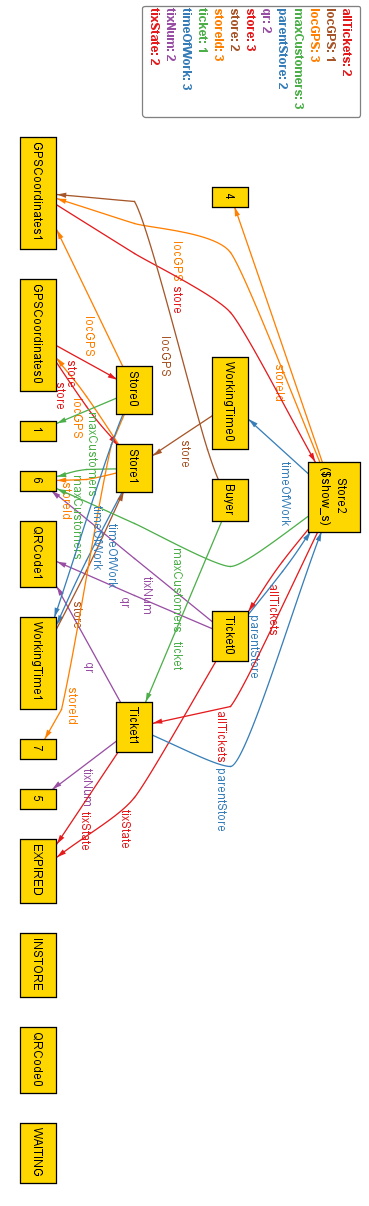
\includegraphics[width=0.38\textwidth]{Images/AlloyGraph1V}
\caption{\label{fig:alloy1}\textbf{Alloy graph 1}}
\end{figure}

\newpage

\begin{figure}[!htb]
\centering
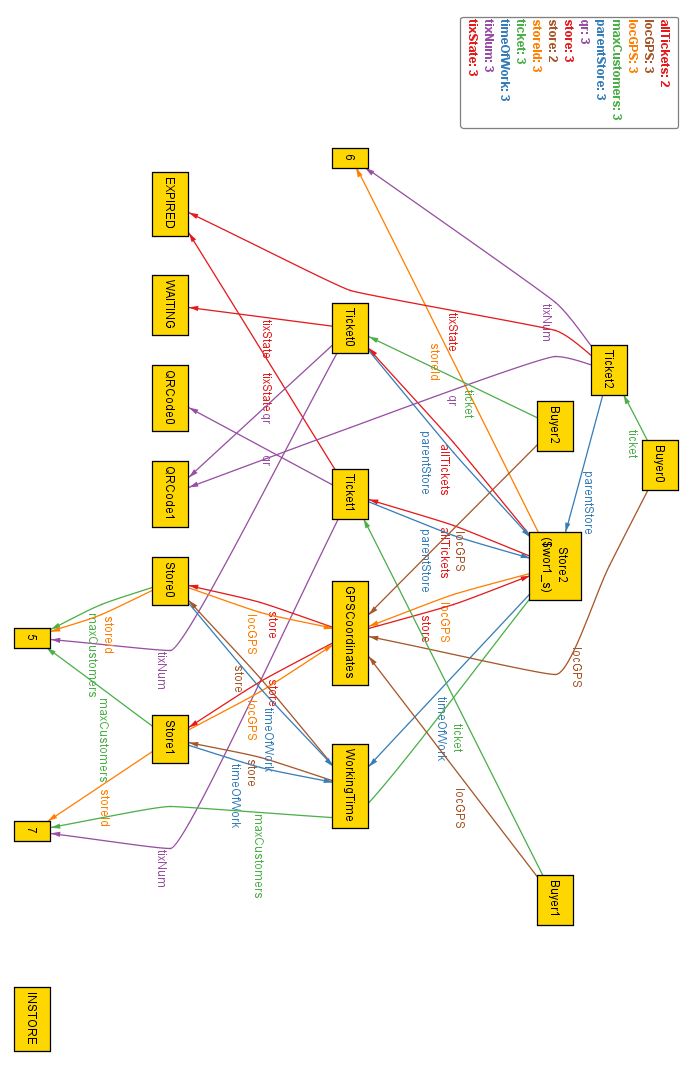
\includegraphics[width=0.8\textwidth]{Images/AlloyGraph2V}
\caption{\label{fig:alloy2}\textbf{Alloy graph 2}}
\end{figure}